\documentclass[colorlinks,empty,plainparagraph]{goose-article}

\usepackage{newfloat}
\usepackage{framed}
\usepackage[most]{tcolorbox}
\usepackage{stfloats}

\title{The onset of fracture in a dual-phase steel}

\author{Tom de Geus}

\hypersetup{pdfauthor={T.W.J. de Geus}}

\newcommand{\TG}[1]{\textcolor{red}{[#1]}}

\begin{document}

\twocolumn[
    \begin{@twocolumnfalse}
        \maketitle
    \end{@twocolumnfalse}
]
\sloppy

\paragraph*{Impact.}

A key to a successful design is to anticipate failure.
In practice it is desirable that failure limits be known material properties, and that approaching the failure limit is accompanied by a clear signal.
This is the case for ductile materials, e.g.\ many crystalline metals, in which significant plastic deformation precedes failure.
Yet, ductility comes at the cost of strength, often resulting in overly bulky (i.e.\ heavy) designs.
To go beyond this trade-off, the next step is to use multiphase materials.
Such materials consist of two or more constituents, each with their own properties.
A significant challenge is that failure of such materials is structurally complex and often very poorly understood.
I propose that that there is a long-range arrangement of constituents responsible for ``soft spots'' that are particularly close to failure, and in which failure is initiated before macroscopic necking occurs.

\paragraph*{Material.}

A material in demand is dual-phase steel, which is widely applied e.g.~in car bodies, as it is strong \emph{and} ductile (as opposed to conventional steels which are strong \emph{or} ductile).
The microstructure comprises grains of two phases: one hard but relatively brittle (martensite) and one soft and ductile (ferrite).

% From deGeus2015a
\begin{figure*}[b]
    \centering
    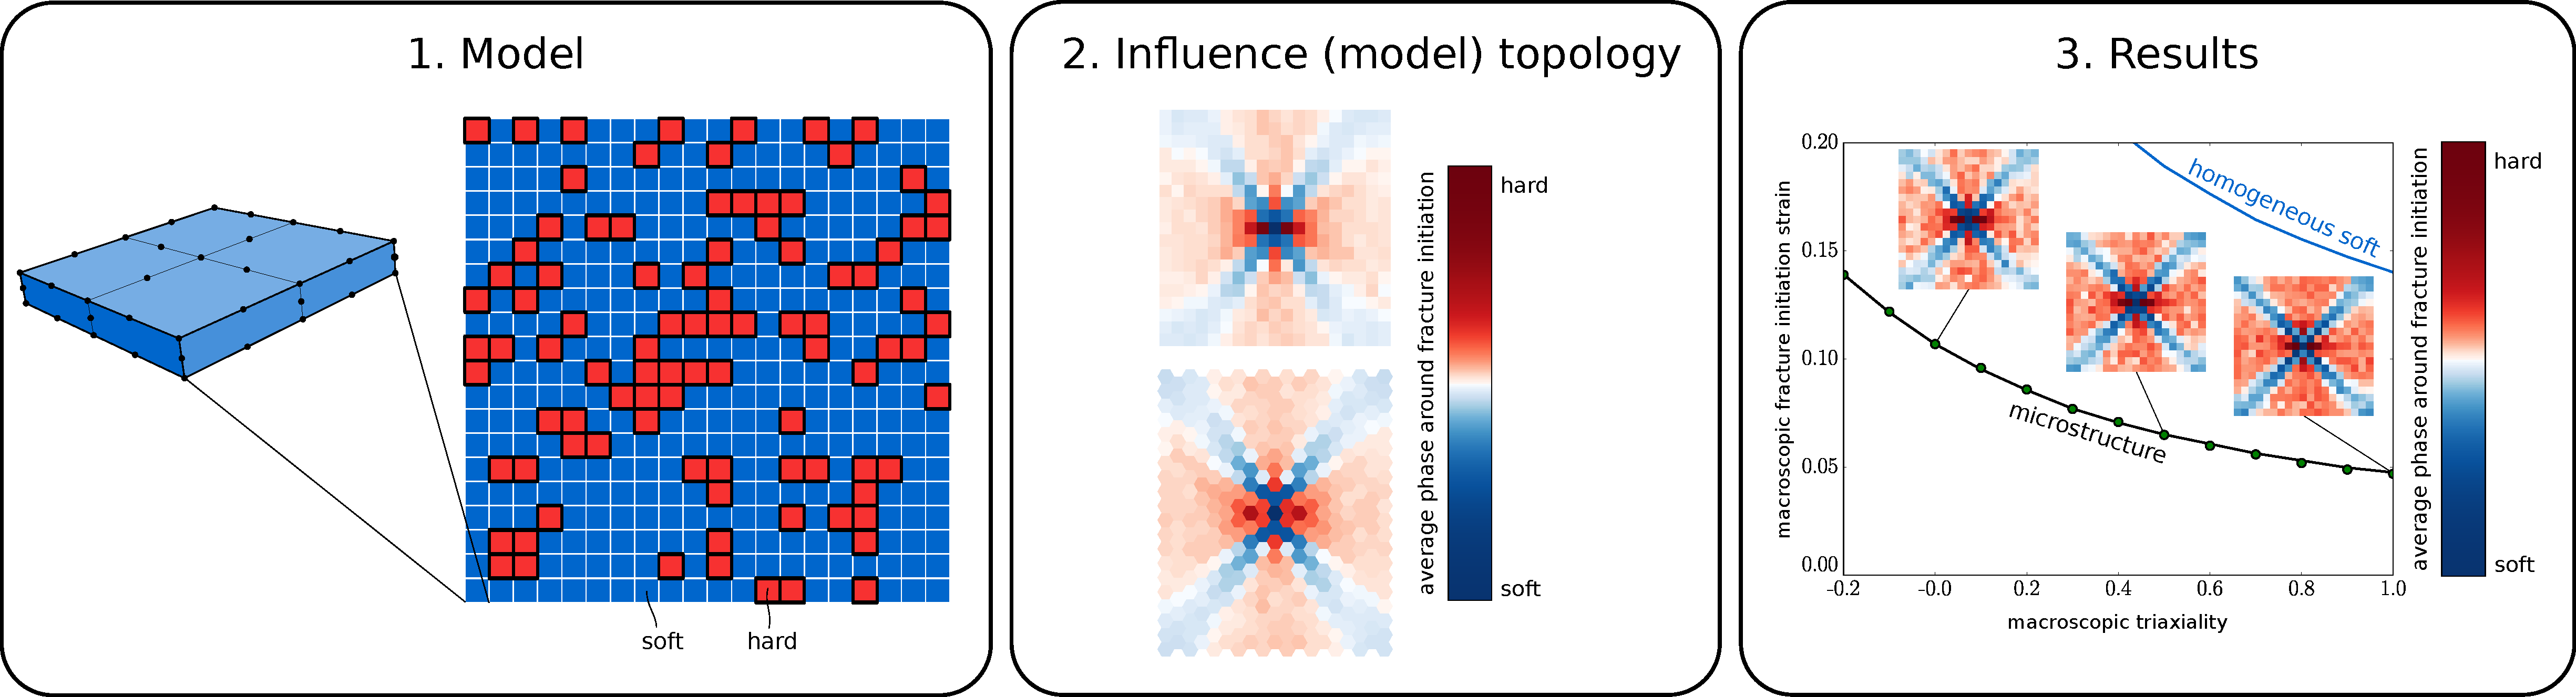
\includegraphics[width=\linewidth]{graphical_abstract.pdf}
\end{figure*}

\paragraph*{Model.}

An abstract model of the microstructure of the dual-phase steel is to assume that it consists of blocks that represent the grains of each phase.
The simplest assumption is that each block is randomly assigned the properties of one of the two phases according to a given volume fraction.
A realisation is presented below (on the left).

\paragraph*{Stress fluctuations.}

Imagine that both phases are elastoplastic and differ only in yield and failure stress.
The non-uniform spatial arrangement leads to a non-uniform plastic deformation such that the tangent modulus is distributed and evolving.
Its impact on failure is consequential.

\paragraph*{Where does failure initiate?}

To answer this question, the microstructure is loaded to a finite strain well before macroscopic fracture.
The answer then comes from computing the average phase around damaged regions.
The result is shown below: Damage initiation occurs where regions of the hard phase, aligned with tension, are interrupted by bands of the soft phase in the directions of shear.
The hard phase triggers high hydrostatic tensile stresses, while giving sufficient room for the shear bands in the soft phase resulting in a high plastic strain.
The results of the two- and three-dimensional models, different geometries, and different loading paths are qualitatively consistent, see e.g.~below.

\nocite{deGeus2016d,deGeus2016a,deGeus2017}

\bibliographystyle{unsrtnat}
\renewcommand{\refname}{Selection of publications}
\bibliography{library}

\end{document}
